\documentclass[11pt]{article}

\usepackage{epsf}
\usepackage{epsfig}
\usepackage{url}
\usepackage{6829hw}

\newcommand{\newc}{\newcommand}

\newc{\code}[1]{{\tt #1}}
\newc{\func}[1]{{\em #1\/}}

\newc{\be}{\begin{enumerate}}
\newc{\ee}{\end{enumerate}}

\newc{\bi}{\begin{itemize}}
\newc{\ei}{\end{itemize}}

\newc{\bd}{\begin{description}}
\newc{\ed}{\end{description}}

\newc{\ov}[1]{$\overline{#1}$}
\newc{\instr}{\tt}

\newc{\doublespace}{\renewcommand{\baselinestretch}{1.5}}

\newcommand{\figref}[1]{Figure~\ref{#1}}
\newcommand{\tref}[1]{Table~\ref{#1}}

% Captioned table
\newc{\tbl}[3]{
        \begin{table}[htb]
                \centering
                #1
                \caption{#3}
                \label{#2}
        \end{table}
}

% Input a table.
\newcommand{\dblfig}[3]{
        \begin{figure}[htb]
		\centering
                \input{#1}
                \caption{#3}
                \label{#2}
        \end{figure}
}

\newcommand{\ddblfig}[4]{
        \begin{figure}[htb]
		\hspace{-0.1in}
                \psfig{figure=#1,width=0.45\textwidth}
                \caption{#3}
                \label{#2}
        \end{figure}
}

% Figure with no caption
\newcommand{\nofig}[2]{
        \begin{figure}[htb]
                \centering
                \psfig{figure=#1}
                \label{#2}
        \end{figure}
}

% Whole page figure
\newcommand{\schfig}[3]{
        \begin{figure}[p]
                \centering
                \psfig{figure=#1,height=7in}
                \caption{#3}
                \label{#2}
        \end{figure}
}

% Small figure
\newcommand{\sfig}[3]{
        \begin{figure}[ltb]
                \centering
               \hspace*{\fill}\rule{\linewidth}{.5mm}\hspace*{\fill}\vspace{3mm}
                \psfig{figure=#1,width=0.4\textwidth}
                \caption{#3}
                \label{#2}
               \vspace{3mm}\hspace*{\fill}\rule{\linewidth}{.5mm}\hspace*{\fill}
        \end{figure}
}

% Medium figure
\newcommand{\mfig}[3]{
        \begin{figure}[ltb]
		\centering
               \hspace*{\fill}\rule{\linewidth}{.5mm}\hspace*{\fill}\vspace{1mm}
                \psfig{figure=#1,height=2.5in}
                \caption{#3}
                \label{#2}
               \vspace{0mm}\hspace*{\fill}\rule{\linewidth}{.5mm}\hspace*{\fill}
        \end{figure}
}

\newcommand{\widefig}[4]{
        \begin{figure*}[htb]
                \centering
               \hspace*{\fill}\rule{\linewidth}{.5mm}\hspace*{\fill}\vspace{5mm}
                \psfig{figure=#1,width=#3}
                \caption{#4}
                \label{#2}
               \vspace{5mm}\hspace*{\fill}\rule{\linewidth}{.5mm}\hspace*{\fill}
        \end{figure*}
}

\newcommand{\mcfig}[4]{
        \begin{figure}[htbp]
                \centering
               \hspace*{\fill}\rule{\linewidth}{.5mm}\hspace*{\fill}\vspace{5mm}
                \psfig{figure=#1,width=#3}
                \caption{#4}
                \label{#2}
               \vspace{5mm}\hspace*{\fill}\rule{\linewidth}{.5mm}\hspace*{\fill}
        \end{figure}
}

\newcommand{\docfig}[3]{
        \begin{figure}[htbp]
               \hspace*{\fill}\rule{\linewidth}{.5mm}\hspace*{\fill}\vspace{5mm}
                \centering
                \psfig{figure=#1,width=#3}
                \label{#2}
               \vspace{5mm}\hspace*{\fill}\rule{\linewidth}{.5mm}\hspace*{\fill}
        \end{figure}
}

% Medium-large figure
\newcommand{\mlfig}[3]{
        \begin{figure}[htb]
                \centering
               \hspace*{\fill}\rule{\linewidth}{.5mm}\hspace*{\fill}\vspace{5mm}
                \psfig{figure=#1,height=3.25in}
                \caption{#3}
                \label{#2}
               \vspace{5mm}\hspace*{\fill}\rule{\linewidth}{.5mm}\hspace*{\fill}
        \end{figure}
}

% Large figure
\newcommand{\lfig}[3]{
        \begin{figure}[p]
                \centering
               \hspace*{\fill}\rule{\linewidth}{.5mm}\hspace*{\fill}\vspace{5mm}
                \psfig{figure=#1,height=5in}
                \caption{#3}
                \label{#2}
               \vspace{5mm}\hspace*{\fill}\rule{\linewidth}{.5mm}\hspace*{\fill}
        \end{figure}
}

% 'gg' figures are the double column versions of the 'g' figures above.
\newcommand{\sfigg}[3]{
        \begin{figure*}[htb]
                \centering
               \hspace*{\fill}\rule{\linewidth}{.5mm}\hspace*{\fill}\vspace{5mm}
                \psfig{figure=#1,height=1.5in}
                \caption{#3}
                \label{#2}
               \vspace{5mm}\hspace*{\fill}\rule{\linewidth}{.5mm}\hspace*{\fill}
        \end{figure*}
}

% Medium figure
\newcommand{\mfigg}[3]{
        \begin{figure*}
                \centering
               \hspace*{\fill}\rule{\linewidth}{.5mm}\hspace*{\fill}\vspace{5mm}
                \psfig{figure=#1,width=\linewidth}
                \caption{#3}
                \label{#2}
               \vspace{0mm}\hspace*{\fill}\rule{\linewidth}{.5mm}\hspace*{\fill}
        \end{figure*}
}

% Medium-large figure
\newcommand{\mlfigg}[3]{
        \begin{figure*}[htb]
                \centering
               \hspace*{\fill}\rule{\linewidth}{.5mm}\hspace*{\fill}\vspace{5mm}
                \psfig{figure=#1,height=3.25in}
                \caption{#3}
                \label{#2}
               \vspace{5mm}\hspace*{\fill}\rule{\linewidth}{.5mm}\hspace*{\fill}
        \end{figure*}
}

% Large figure
\newcommand{\lfigg}[3]{
        \begin{figure*}[p]
                \centering
               \hspace*{\fill}\rule{\linewidth}{.5mm}\hspace*{\fill}\vspace{5mm}
                \psfig{figure=#1,height=5in}
                \caption{#3}
                \label{#2}
               \vspace{5mm}\hspace*{\fill}\rule{\linewidth}{.5mm}\hspace*{\fill}
        \end{figure*}
}

% Variable size figure
\newcommand{\vfigg}[4]{
        \begin{figure*}[htb]
                \centering
               \hspace*{\fill}\rule{\linewidth}{.5mm}\hspace*{\fill}\vspace{5mm}
                \psfig{figure=#1,#2}
                \caption{#4}
                \label{#3}
               \vspace{5mm}\hspace*{\fill}\rule{\linewidth}{.5mm}\hspace*{\fill}
        \end{figure*}
}

\newcommand{\vfig}[4]{
        \begin{figure}[ltb]
                \centering
               \hspace*{\fill}\rule{\linewidth}{.5mm}\hspace*{\fill}\vspace{1mm}
                \psfig{figure=#1,#2}
                \caption{#4}
                \label{#3}
               \vspace{1mm}\hspace*{\fill}\rule{\linewidth}{.5mm}\hspace*{\fill}
        \end{figure}
}

\newcommand{\vnlfig}[4]{
        \begin{figure}[htb]
                \centering
               \hspace*{\fill}\rule{\linewidth}{0mm}\hspace*{\fill}\vspace{5mm}
                \psfig{figure=#1,#2}
                \caption{#4}
                \label{#3}
               \vspace{0mm}\hspace*{\fill}\rule{\linewidth}{0mm}\hspace*{\fill}
        \end{figure}
}

\newcommand{\dblvfig}[6]{
        \begin{figure}[htb]
                \centering
                \hspace*{\fill}\rule{\linewidth}{0mm}\hspace*{\fill}\vspace{0.5mm}
                \psfig{figure=#1,#2}
	        \hspace{1in}
                \psfig{figure=#3,#4}
                \caption{#6}
                \label{#5}
               \vspace{2mm}\hspace*{\fill}\rule{\linewidth}{0mm}\hspace*{\fill}
        \end{figure}
}
\newc{\myspacing}{
        \let\oldtextheight=\textheight
        \let\oldtextwidth=\textwidth

        \let\oldtopmargin=\topmargin
        \let\oldheadheight=\headheight
        \let\oldfootheight=\footheight
        \let\oldheadsep=\headsep
        \let\oldoddsidemargin=\oddsidemargin


        \textheight 8.5in
        \textwidth 6in

        \topmargin 0in
        \headheight 0in
        \footheight 1.5in
        \headsep 0in
        \oddsidemargin 0in

}

\newc{\oldspacing}{
        \let\textheight=\oldtextheight 
        \let\textwidth=\oldtextwidth

        \let\topmargin=\oldtopmargin 
        \let\headheight=\oldheadheight 
        \let\footheight=\oldfootheight
        \let\headsep=\oldheadsep
        \let\oddsidemargin=\oldoddsidemargin
}
% Local Variables: 
% mode: latex
% TeX-master: t
% End: 


\begin{document}

\newcounter{listcount}
\newcounter{sublistcount}


\handout{H1}{January 14, 2013}{Instructor: Prof. Nick Feamster}
{College of Computing, Georgia Tech}{Problem Set 1: Link Layer and
  IP} 

%This problem set has three questions, each with several parts.  Answer
%them as clearly and concisely as possible.  You may discuss ideas with
%others in the class, but your solutions and presentation must be your
%own.  Do not look at anyone else's solutions or copy them from
%anywhere. (Please refer to the Georgia Tech honor code, posted on the
%course Web site).

Turn in your writeup and talk on {\bf January 28, 2013} by 11:59pm.
{\em Please upload your solutions to T-Square.  Other forms of
  submission will not be accepted!}  We will be providing more
information about how to turn in your assignment as the due date
approaches.

\section{Learning (about) Bridges}

\begin{figure}[h]
\centering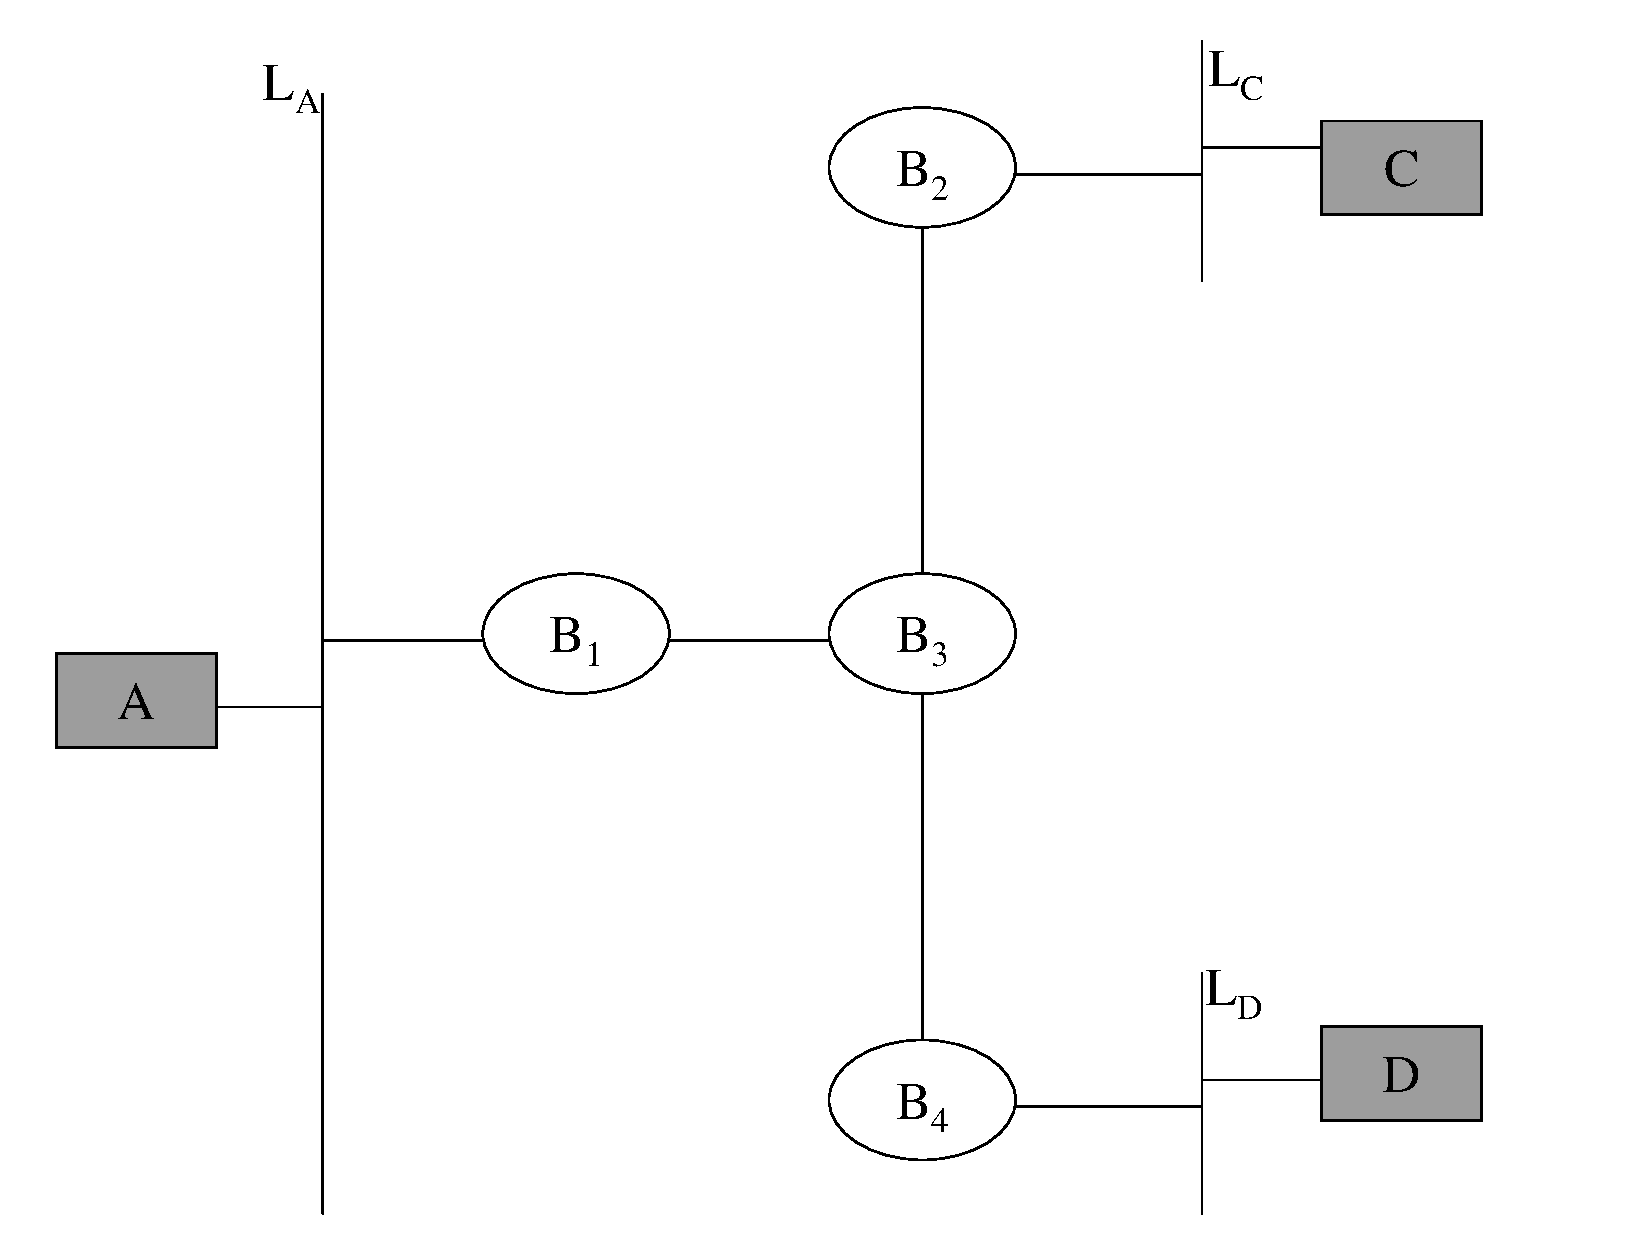
\includegraphics[height=2.5in]{ps1-bridge}
\label{f:ps1-bridge}
\caption{Bridge topology.}
\end{figure}

Consider the bridge topology shown in Figure~\ref{f:ps1-bridge}.
Assuming that all of the forwarding tables are initially empty, write
out the forwarding tables at each of the four bridges $B1$ through $B4$
at the conclusion of the following transmissions:

\begin{enumerate}
\item $D$ sends to $A$
\item $A$ sends to $D$
\item $C$ sends to $A$
\end{enumerate}

In the forwarding table at each note, identify the port by the unique
LAN segment ($L_A$, $L_C$, or $L_D$) reachable using that port, unless
there isn't one, in which case use the identifier of the neighboring
bridge to identify the port.

\newpage

\section{Circuit Switching vs. Packet Switching}

Consider a typical dormitory network, where hundreds of users (and
devices) might share a 10~Gbps link to the rest of the campus network.
Each user alternates between periods of activity and inactivity.  During
periods of activity (where a user may be checking email, browsing the
Web, watching videos, and swapping files), suppose each user creates a
demand of 200~Mbps.  During periods of inactivity, suppose (for
simplicity) that the user generates no data.

\paragraph{Circuit Switching}
\begin{enumerate}
\item With circuit switching, 200~Mbps must be reserved for each user at
  all times.  Suppose that a one-second TDM frame is divided into 10
  time slots of 100~ms each.  How many simultaneous users can the
  circuit switched network support?
\item Suppose that a typical dorm room has 500 users.  What is the
  probability that at least one user gets a ``busy signal'' with a
  circuit switched network (i.e., what is the probability that the
  number of active users exceeds the number of users that you calculated
  in part~1)?
\item Plot the probability of a ``busy signal'' as a function of the
  number of users in the dorm.  In other words, show a plot with your
  answer from part~2, but varying the number 500 from zero to
  2,000. What do you observe?
\end{enumerate}

\paragraph{Packet Switching}
\begin{enumerate}
\item Describe the advantages and disadvantages of packet switching with
  respect to circuit switching.
\item Suppose that users are sending traffic through a single router
  with an M/M/1 queue (look it up).  Suppose that on average, there are
  300 active users, each of which send about 10~Mbps {\em on average}
  (note that this accounts for peaks).  Suppose that, as before, the
  average service rate of the link is 10~Gbps.  What is the average
  delay seen by any given packet?
\item Suppose that a packet traverses five links with similar delay
  characteristics as it travels from Atlanta to San Francisco.  What is
  the expected {\em total} delay experienced by each packet?  {\em
    Clearly show your work, accounting for queueing delay, transmission
    delay, and propagation delay.}  Assume that there is no processing
  delay.
\item Run a {\tt ping} command from your computer at Georgia Tech (or
  somewhere in Atlanta) to {\tt www.cs.stanford.edu}; this shows {\em
    round trip delay}.  Show the output.  Does this reconcile with your
  back-of-the-envelope calculations from the previous part?  Why or why
  not?
\end{enumerate}

\pagebreak

\section{Fun with ARP}

This problem is a quick ``hands on'' assignment to get you familiar with
ARP.  For this problem, you will need access to a machine that has the {\tt
  arp} command, as well as some kind of packet-capture capability (e.g.,
{\tt tcpdump} or {\tt ethereal}).

\begin{enumerate}
\item At your command prompt, type {\tt arp -a} or equivalent.  You
  should see a line that looks something like this:
\begin{quote}
cc-cisco-143out4.cc.gt.atl.ga.us (143.215.131.1) at 0:16:9c:fd:98:0 on en0 ifscope [ethernet]
%cc-cisco-143out2.cc.gt.atl.ga.us (143.215.129.1) at 00:08:20:db:1d:80 [ether] on eth0
\end{quote}
\begin{itemize}
\item What is the IP address on this line?  
\item What is the MAC address referring to?  
\item What does 'en0' mean?
\end{itemize}
\item Now, issue your own ARP request with the {\tt arp} command.  Make
  an ARP request for whatever IP address you found in your ARP table
  from the first part of the problem.  Turn in the command that you
  used to generate this request.
\item {\em Packet capture.} Use a packet capture program (e.g., {\tt
  ethereal}, {\tt wireshark}) to capture the ARP requests that you can
  see on your network.  {\em In your writeup, show a screenshot (or text
  output) of your captured ARP packets.}
\begin{itemize}
\item Why do you see ``who-has'' ARP requests from other machines that
  are not yours?
\item How often do you see an ARP request from your machine, or any
  other machine on the network?  Why do you see these requests
  repeatedly?  (Hint: Think about the discussion of ``fate sharing''
  from lecture.)
\end{itemize}
\end{enumerate}

\pagebreak

\section{IP Addresses}

This problem is a ``hands on'' assignment to help you learn about
Internet address registries.  You will use the {\tt whois} command-line
tool. {\bf Type ``{\tt whois -h whois.arin.net '?'}'' for help using this tool.}

\begin{enumerate}
\item What is the current IP address for your computer from which you
  are doing this assignment? Explain how you got this information (there
  are several ways to do it).
\item What is the CIDR prefix range for the IP address you found from
  Part 1?
\item If you do this portion of the assignment from Georgia Tech, you
  will see something called ``Direct Assignment'' when you look up the
  IP address.  What does that mean?
\item What is the AS number for the IP address that you looked up?
  Explain how autonomous system numbers are assigned, and how they are
  used.
\item Look up the following IP addresses.  For each, give the IP prefix
  associated with the allocated IP adddress, and {\em
  entire allocations chain}, as well as the current owner of the prefix
  (i.e., the list of registries through which the prefix was
  allocated). {\em Include sub-allocations, including the size of each
    sub-allocation.} 
\begin{itemize}
\item 41.132.75.118
\item 204.77.224.9
\item 76.88.123.65
\item 99.151.0.68 
\end{itemize}
\end{enumerate}

\section{IP Address Exhaustion and IPv6}


Skim through Geoff Huston's article from the January 2013 {\em ISP Column}:
\url{http://www.potaroo.net/ispcol/2013-01/2012.html}.  

Huston says: ``The past three years has been dominated by the mass
marketing of mobile internet services, and the growth rates for 2012
perhaps might have been the highest so far recorded were it not for the
exhaustion of the IPv4 address pools in the Asia Pacific region and
Europe and the Middle East. In address terms this growth is being masked
by the use of Carrier Grade NATs in the mobile service provider
environment, so that the resultant demands for public addresses in IPv4
are quite low. In theory there is no such requirement for IPv6 to use
NATS, and if the mobile world were deploying dual stack ubiquitously
then this would be evident in the IPv6 address allocation data.''

\begin{enumerate}
\item How is it possible for ISPs to keep adding customers if we are
  ``out of IPv4 addresses''?  (Explain this paradox.)
\item What is ``Carrier Grade NAT''?
\item Describe the advantages and disadvantages of using NAT vs. IPv6 in
  terms of both functionality and potential to curb address space
  exhaustion.
\item Table 13 shows the largest IPv6 organizations by organization in
  2012, in terms of /32 allocations.  How many addresses is a /32
  allocation, in IPv6?  
\end{enumerate}


\section{Book Problems}

Please complete the following problems from Kurose and Ross, 6th
Edition:

\begin{enumerate}
\itemsep=-1pt
\item {\em Access Networks.} R6, R9
\item {\em Delays and Throughput.} P24, P25

\end{enumerate}



\end{document}
